\subsection{Cấu trúc thật của luồng khí trong môi trường có gió}
Trực giác thông thường hình dung một nguồn phát khí tạo ra một đám mây hình nón mịn, nồng độ cao nhất ở tâm và giảm đều ra ngoài. Hình ảnh đó \textbf{đúng với nồng độ trung bình theo thời gian}, nhưng \textbf{sai với giá trị tức thời} --- mà giá trị tức thời mới là thứ một cảm biến trên robot đọc được.

Murlis, Elkinton và Cardé tổng kết các phép đo cấu trúc thật của luồng mùi trong bài tổng quan trên \textit{Annual Review of Entomology} năm 1992 [1]. Trong dòng khí có gió, chất khí bị rối loạn xé thành các cụm rời rạc xen kẽ với những khoảng không khí gần như sạch. Hai kết quả trong bài đặc biệt quan trọng đối với đề tài này.

Thứ nhất, \textbf{độ dài các đợt khí trải trên một dải rất rộng}. Nguyên văn, trang 516:

\begin{trichdan}
``Bursts last from less than 10 ms to over a second and burst return periods from 500 ms to several minutes.''
\end{trichdan}
Thứ hai, và đây là kết quả quyết định, ở trang 517:

\begin{trichdan}
``Distributions of burst-peak concentrations from signals recorded at different positions overlapped significantly, even when they were as much as 5 m apart.''
\end{trichdan}
Nghĩa là: phân bố nồng độ đỉnh đo tại hai vị trí \textbf{cách nhau tới 5 mét} vẫn chồng lấn lên nhau đáng kể. Cùng bài còn dẫn phép đo của Storebø và cộng sự, tìm thấy những mảng khí gần như chưa bị pha loãng ở cách nguồn từ 100 mét trở lên.

Phần tóm tắt của bài, trang 526, cô đọng toàn bộ vấn đề trong một câu:

\begin{trichdan}
``Odor signals consist of short bursts of odor of greatly varying intensity. Farther from the source, bursts are on average weaker (but not reliably so).''
\end{trichdan}
Bốn chữ trong ngoặc --- \textit{``but not reliably so''} --- là điểm mấu chốt. Càng xa nguồn thì các đợt khí \textbf{trung bình} có yếu đi, nhưng quan hệ đó \textbf{không đáng tin cậy} ở mức từng phép đo. Hệ quả trực tiếp: \textbf{một phép đo nồng độ đơn lẻ không cho biết robot đang ở gần hay xa nguồn.} Đại lượng giảm đều theo khoảng cách là nồng độ trung bình theo thời gian, trong khi robot chỉ có giá trị đọc tại một thời điểm.

\begin{ghichu}
Cần nói rõ một điểm về phạm vi áp dụng: mức độ đứt quãng của luồng khí không phải hằng số, nó phụ thuộc vào tỉ lệ giữa kích thước nguồn phát và kích thước các xoáy rối. Chính bài tổng quan [1] dẫn hai kết quả trái chiều: trong ống gió, Fackrell và Robins thấy độ đứt quãng giảm dần theo khoảng cách và gần bằng không ở xa xuôi gió; còn ngoài khí quyển, nơi nguồn phát nhỏ hơn xoáy rối, Mylne và Mason thấy độ đứt quãng luôn giữ ở mức lớn hơn không. Sân thử nghiệm 2 m trong phòng của nhóm nằm giữa hai chế độ đó, và nhóm \textbf{chưa đo được} nó thuộc về bên nào. Vì vậy báo cáo này trình bày kết quả dưới dạng \textbf{thứ hạng giữa ba thuật toán trên cùng một trường khí}, không dưới dạng con số tuyệt đối có thể ngoại suy ra thực địa.
\end{ghichu}

\subsection{Nguyên lý cảm biến khí oxit kim loại và cảm biến MQ-3}

\subsubsection{Nguyên lý hoạt động}
Bên trong cảm biến MQ-3 có một lớp thiếc đi-ô-xít (SnO$_{2}$) được nung nóng liên tục bằng một sợi đốt. Trong không khí sạch, oxy hấp phụ lên bề mặt lớp bán dẫn này và giữ lấy electron dẫn, làm lớp bán dẫn dẫn điện kém --- tức là \textbf{điện trở cao}. Khi hơi cồn tiếp xúc bề mặt, nó phản ứng với lớp oxy hấp phụ và trả electron về lớp bán dẫn, làm \textbf{điện trở giảm xuống}.

Điểm cần nhấn mạnh: \textbf{cảm biến không đo nồng độ. Nó chuyển nồng độ thành một điện trở.} Toàn bộ phần còn lại là công việc của mạch điện và phần mềm.


\subsubsection{Từ điện trở tới nồng độ ước lượng}
Trên module, lớp nhạy khí (điện trở Rs) mắc nối tiếp với một điện trở tải RL cố định, tạo thành mạch chia áp. Từ điện áp đo được suy ngược ra Rs:

\[ V_{\text{out}} = V_c\,\frac{R_L}{R_s+R_L} \qquad\Longrightarrow\qquad R_s = R_L\,\frac{V_c - V_{\text{out}}}{V_{\text{out}}} \]
Giá trị Rs tuyệt đối không dùng trực tiếp được, vì hai con MQ-3 cùng lô sản xuất có thể chênh nhau vài lần. Datasheet vì vậy không vẽ đặc tuyến theo Rs mà theo \textbf{tỉ số Rs/R$_{0}$}, trong đó R$_{0}$ là một điện trở tham chiếu của chính con cảm biến đó --- tỉ số triệt tiêu được sự khác nhau giữa các con.

Cần định nghĩa R$_{0}$ cho đúng. Datasheet MQ-3 ghi nguyên văn:

\begin{trichdan}
``Rs means resistance in different gases, Ro means resistance of sensor in 0.4mg/l alcohol''
\end{trichdan}
Nghĩa là R$_{0}$ \textbf{không phải} điện trở trong không khí sạch, mà là điện trở tại một nồng độ cồn chuẩn 0,4 mg/L. Nhóm không có điều kiện tạo chính xác nồng độ đó, nên dùng một đường vòng đọc từ chính đồ thị đặc tuyến: đường ứng với không khí sạch nằm tại Rs/R$_{0}$ = 60. Do đó:

\[ R_0 = \frac{R_s(\text{đo trong không khí sạch})}{60} \]
Con số 60 vì vậy cũng là \textbf{một số đọc từ đồ thị}, và điều này được ghi nhận thẳng thắn trong phần hạn chế. Firmware đo lại R$_{0}$ mỗi lần khởi động để bám theo điều kiện nhiệt độ, độ ẩm của phòng tại thời điểm chạy.

Bước cuối là đường đặc tuyến luỹ thừa:

\[ \text{ppm} = A\left(\frac{R_s}{R_0}\right)^{\!B} \qquad\text{với } A = 315{,}2 \text{ và } B = -1{,}865 \]
Hai hệ số A và B được fit từ \textbf{hai điểm đọc trên đồ thị ethanol của datasheet}: tại 0,1 mg/L thì Rs/R$_{0}$ = 2,6; tại 10 mg/L thì Rs/R$_{0}$ = 0,22. Quy đổi ở 25 $^\circ$C, 1 mg/L ethanol tương đương khoảng 531 ppm, nên hai điểm đó là 53,1 ppm và 5310 ppm. Từ hai điểm:

\[ B = \frac{\ln(5310/53{,}1)}{\ln(0{,}22/2{,}6)} = \frac{4{,}605}{-2{,}470} = -1{,}865 \qquad A = \frac{53{,}1}{2{,}6^{-1,865}} = 315{,}2 \]

\subsubsection{Hệ số khuếch đại sai số 1,87}
Đường đặc tuyến trên là một hàm luỹ thừa, tức là \textbf{một đường thẳng trên giấy log--log}, và B chính là độ dốc của đường thẳng ấy. Lấy logarit hai vế rồi vi phân:

\[ \ln(\text{ppm}) = \ln A + B\ln\!\left(\frac{R_s}{R_0}\right) \qquad\Longrightarrow\qquad \frac{d(\text{ppm})}{\text{ppm}} = B\,\frac{d(R_s/R_0)}{R_s/R_0} \]
Vậy \textbf{sai số tương đối của ppm bằng |B| $\approx$ 1,87 lần sai số tương đối của Rs/R$_{0}$}. Cụ thể, nếu phép đo Rs/R$_{0}$ sai 10 \% thì giá trị ppm hiển thị sai khoảng 19 \%. Hình 2.1 minh hoạ điều đó bằng hình học: trên giấy log--log, một sai số phần trăm ở trục ngang là một đoạn dịch ngang có độ dài cố định; vì đường đặc tuyến dốc 1,87 nên đoạn dịch ngang ấy biến thành một đoạn dịch dọc cao gấp 1,87 lần.

\begin{figure}[!htbp]
  \centering
  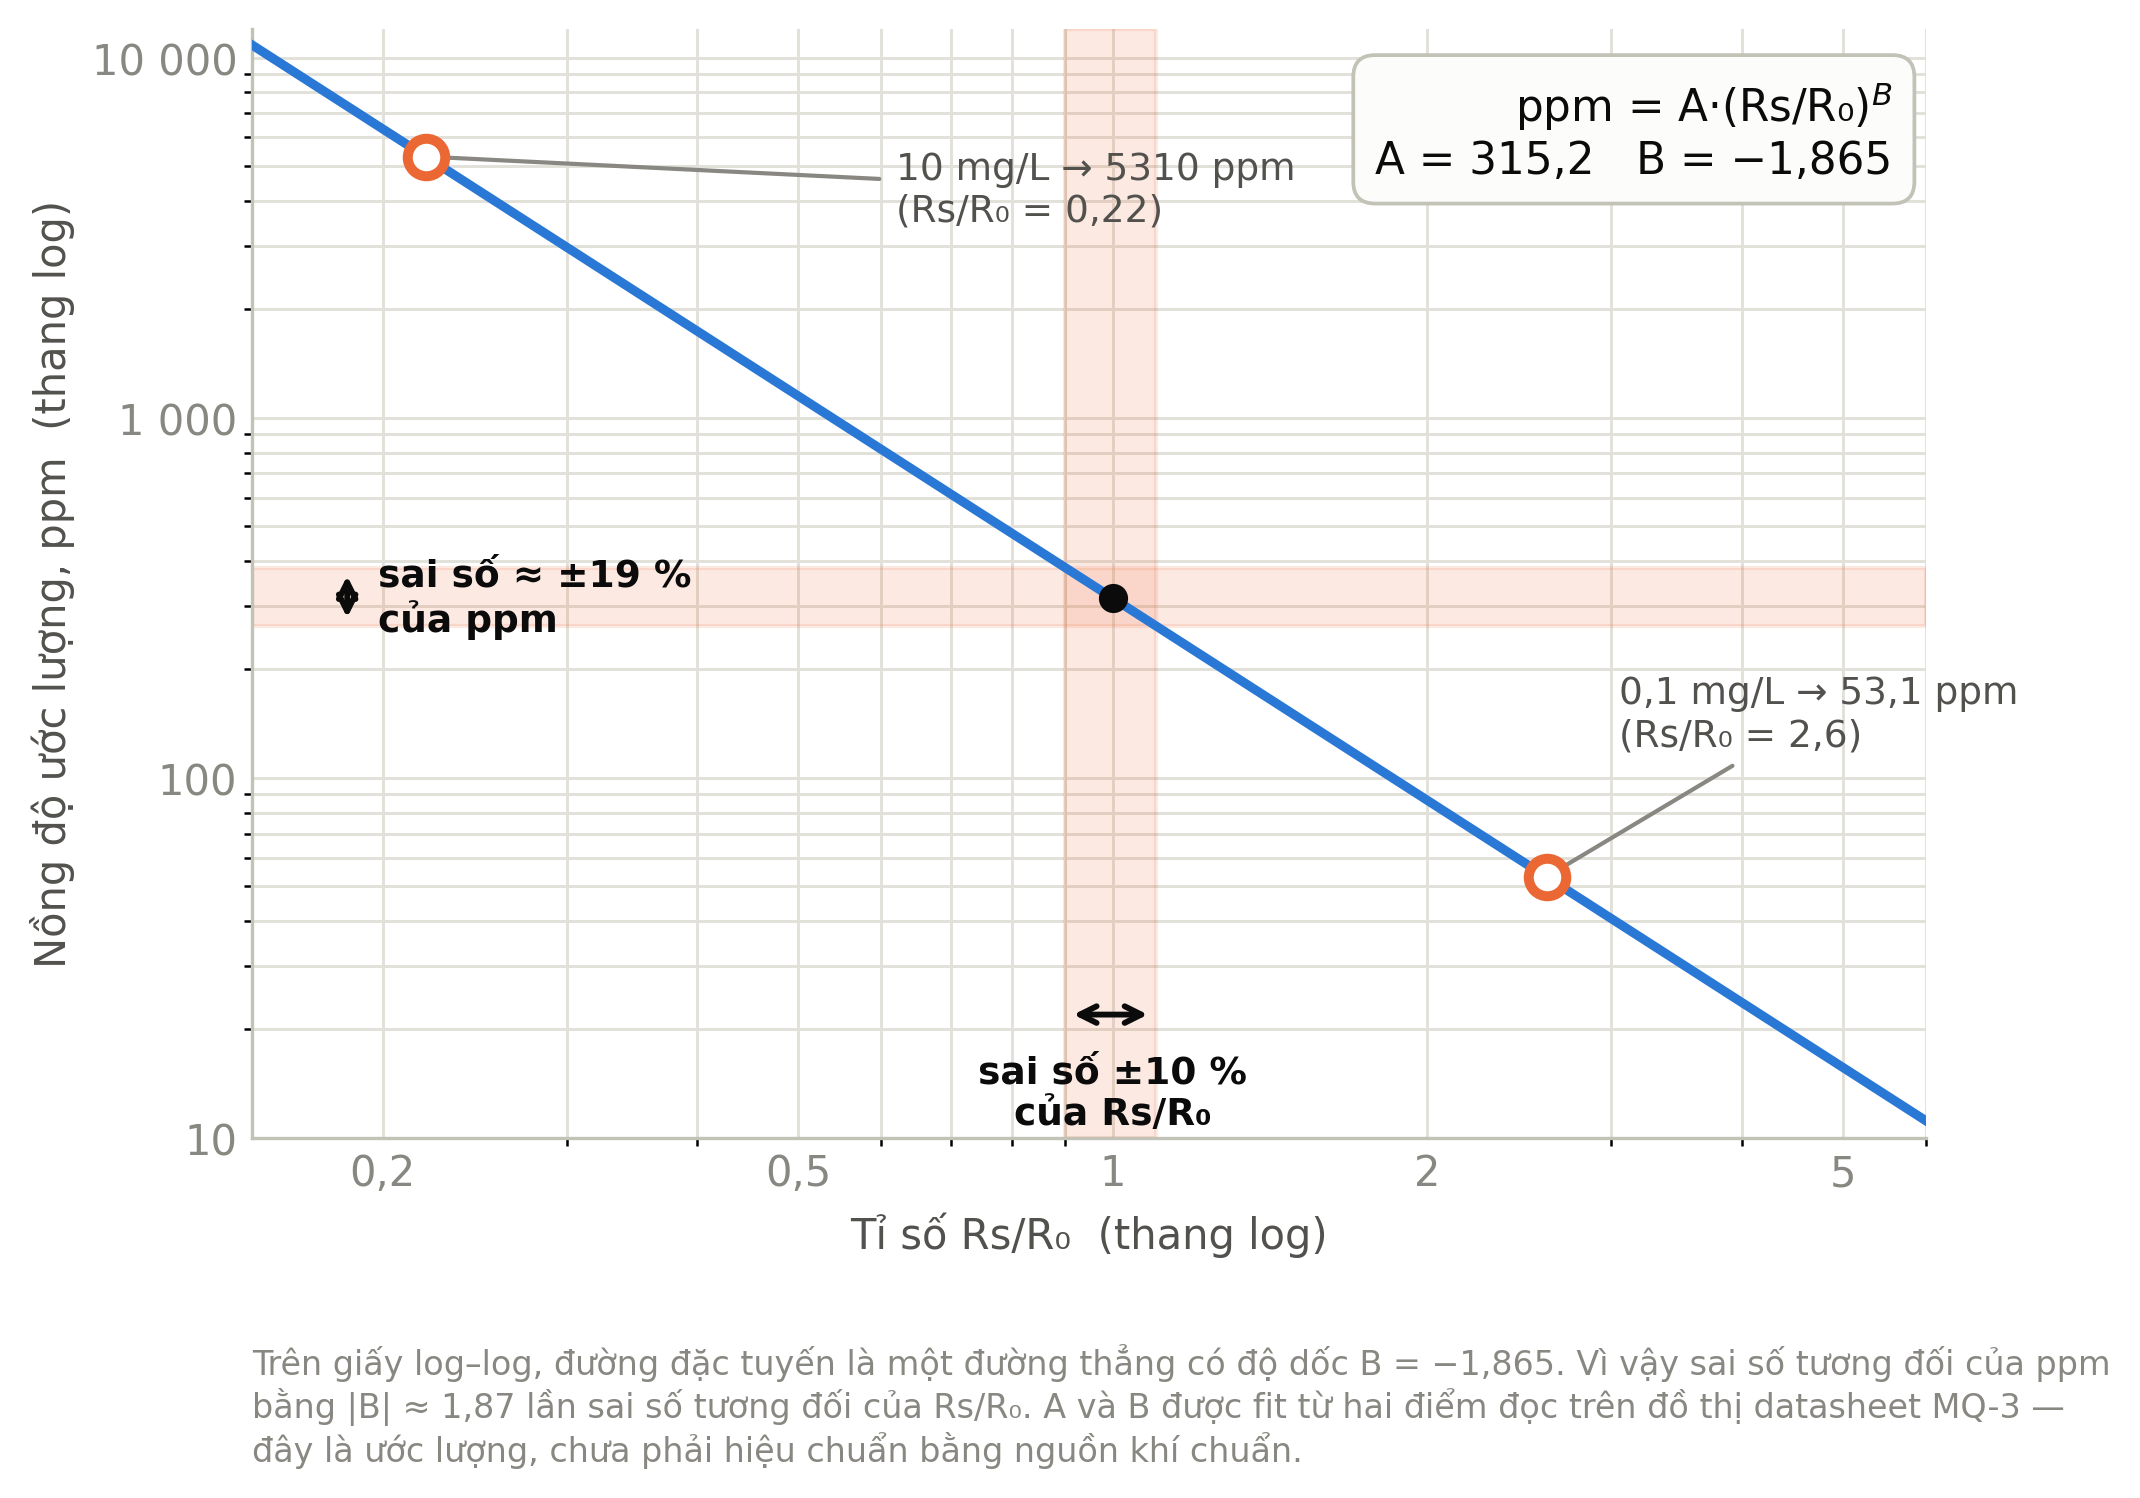
\includegraphics[width=0.882\textwidth]{pic/mq3_dactuyen.png}
  \caption{Đường đặc tuyến MQ-3 trên thang log--log và cơ chế khuếch đại sai số. Độ dốc của đường đặc tuyến chính là hệ số khuếch đại sai số tương đối.}
\end{figure}
Cần nói cho chặt: công thức trên là \textbf{xấp xỉ bậc nhất}, chỉ đúng khi sai số nhỏ. Nếu Rs/R$_{0}$ sai đi một hệ số (1 + δ) thì ppm sai đi đúng bằng (1 + δ)\textsuperscript{B} -- 1; với δ = +10 \%, xấp xỉ tuyến tính cho --18,7 \% còn giá trị chính xác là --16,3 \%. Hai con số cùng bậc độ lớn, nên dùng hệ số 1,87 để nói về \textbf{độ lớn} của sai số là hợp lý, còn nhóm không dùng nó để tính toán chính xác.

\textbf{Kết luận thiết kế rút ra từ con số này.} Vì R$_{0}$ được đo lại mỗi lần bật máy và bản thân nó cũng có sai số; vì A và B chỉ là ước lượng từ hai điểm đọc trên một đồ thị in; và vì mọi sai số ấy còn bị nhân thêm 1,87 lần --- nhóm kết luận rằng \textbf{giá trị ppm tuyệt đối của một cảm biến MQ-3 chưa hiệu chuẩn không đủ tin cậy để dựa vào mà tìm nguồn}. Đây chính là lý do dẫn tới kiến trúc hai lớp dữ liệu trình bày ở mục 4.2: thuật toán tìm nguồn \textbf{chỉ dùng tín hiệu tương đối}, còn giá trị ppm chỉ đi ra màn hình cho người vận hành.


\subsubsection{Vì sao chọn MQ-3 thay vì cảm biến chính xác hơn}
\begin{table}[!htbp]
  \centering
  \caption{So sánh ba họ cảm biến khí ứng viên cho đề tài}
  \small
  \renewcommand{\arraystretch}{1.25}
  \begin{tabular}{>{\raggedright\arraybackslash}p{0.1931\textwidth}>{\raggedright\arraybackslash}p{0.1755\textwidth}>{\raggedright\arraybackslash}p{0.1755\textwidth}>{\raggedright\arraybackslash}p{0.3335\textwidth}}
    \toprule
    \textbf{Tiêu chí} & \textbf{MQ-3 (MOX)} & \textbf{PID} & \textbf{NDIR} \\
    \midrule
    Giá thành & Rất thấp & Cao gấp hàng chục tới hàng trăm lần & Cao \\
    Độ chính xác nồng độ & Thấp khi chưa hiệu chuẩn & Cao & Cao \\
    Thời gian hồi phục & Chậm (hàng chục giây) & Nhanh & Nhanh \\
    Công suất tiêu thụ & Sợi đốt khoảng 750 mW & Thấp hơn & Thay đổi theo loại \\
    Ảnh hưởng tới kết luận của đề tài & \textbf{Không}, vì thuật toán chỉ dùng tín hiệu tương đối & Không & Không \\
    \bottomrule
  \end{tabular}
\end{table}
Bảng 2.1 cho thấy điểm quan trọng nhất nằm ở dòng cuối: các cảm biến chính xác hơn \textbf{không làm thay đổi kết luận của đề tài}, bởi kết luận nằm ở so sánh thuật toán chứ không nằm ở độ chính xác nồng độ. Nhóm thiết kế thuật toán để chỉ cần tín hiệu tương đối, chính là để kết luận không phụ thuộc vào việc dùng cảm biến đắt hay rẻ. Đổi lại, việc chọn cảm biến rẻ và chậm khiến \textbf{độ trễ của cảm biến trở thành ràng buộc thiết kế trung tâm}, và toàn bộ quy trình đo ở mục 4.3 được dựng quanh ràng buộc đó.


\subsection{Độ trễ của cảm biến oxit kim loại}
Cảm biến MOX phản ứng \textbf{bất đối xứng}: nồng độ tăng thì tín hiệu lên tương đối nhanh, nhưng khi khí đi qua thì tín hiệu \textbf{hồi phục rất chậm}. Datasheet MQ ghi thời gian đáp ứng dưới 10 giây và thời gian hồi phục tới 30 giây. Monroy, González-Jiménez và Blanco phân tích chi tiết hiện tượng này trên tạp chí \textit{Sensors} năm 2012 [3]: thời gian hồi phục ở mức hàng chục giây, và khi robot vừa di chuyển vừa đo thì giá trị ổn định ``hiếm khi đạt tới được''. Bài báo gọi hệ quả quan sát được là \textbf{``hiệu ứng đuôi''} --- giá trị cao còn kéo dài dọc theo đường đi rất lâu sau khi robot đã rời khỏi vùng có khí. Giải pháp thường dùng trong tài liệu là giảm tốc độ robot xuống còn vài xentimét mỗi giây.

Hệ quả rất cụ thể cho đề tài: \textbf{nếu đọc cảm biến trong lúc xe đang chạy, con số nhận được ứng với chỗ xe vừa đi qua, chứ không ứng với một vị trí xác định nào cả.} Đây là lý do trực tiếp dẫn tới ba quyết định thiết kế quan trọng nhất của phần mềm, trình bày ở mục 4.3 và 4.7.


\subsection{Vì sao chỉ dùng một cảm biến khí}
Câu hỏi tự nhiên nhất khi nhìn vào đề tài là: nếu muốn biết khí đậm hơn về phía nào, tại sao không gắn hai cảm biến ở hai bên xe rồi so sánh, giống như hai lỗ mũi? Nhóm đã cân nhắc phương án đó và \textbf{loại nó vì lý do vật lý, không phải vì tiết kiệm chi phí}. Lập luận gồm ba lớp.


\subsubsection{Lớp thứ nhất --- bằng chứng thực nghiệm đã công bố}
Kết quả trích ở mục 2.1 đã trả lời gần như trọn vẹn: phân bố nồng độ đỉnh đo tại hai vị trí \textbf{cách nhau tới 5 mét} vẫn chồng lấn lên nhau [1, tr. 517]. Nếu 5 mét còn chưa đủ để phân biệt gần hay xa nguồn bằng nồng độ tức thời, thì hai cảm biến cách nhau khoảng 10--20 cm trên cùng một chiếc xe chắc chắn không đủ.


\subsubsection{Lớp thứ hai --- vì sao tăng khoảng cách hai cảm biến cũng không cứu được}
Gọi khoảng cách giữa hai cảm biến là \textit{d}. Hiệu số hai giá trị đọc được gồm hai thành phần:

\[ \Delta C = C(x+d) - C(x) \]
Thành phần \textbf{tín hiệu} --- phần ta muốn đo --- tỉ lệ với tích của \textit{d} và đạo hàm của nồng độ trung bình theo phương \textit{x}. Thành phần \textbf{nhiễu} --- phần dao động rối --- có độ lệch chuẩn bằng căn bậc hai của biểu thức 2$\sigma$$^{2}$$\cdot$(1 -- $\rho$(d)), trong đó $\sigma$ là biên độ dao động rối và $\rho$(d) là \textbf{hàm tương quan không gian}: hai điểm cách nhau \textit{d} thì giá trị của chúng giống nhau đến mức nào.

Xét đúng trường hợp của đề tài: \textit{d} rất nhỏ so với kích thước đặc trưng của một cấu trúc khí. Khi đó 1 -- $\rho$(d) xấp xỉ tỉ lệ với \textit{d}$^{2}$, nên thành phần nhiễu tỉ lệ với \textit{d}. Mà thành phần tín hiệu \textbf{cũng} tỉ lệ với \textit{d}. Lập tỉ số:

\[ \frac{\text{tín hiệu}}{\text{nhiễu}} \;\approx\; \frac{d\cdot\partial\bar{C}/\partial x}{\sqrt{2\sigma^{2}\bigl(1-\rho(d)\bigr)}} \;\xrightarrow[\;1-\rho(d)\,\propto\,d^{2}\;]{\;d\ll L\;}\; \frac{L\cdot\partial\bar{C}/\partial x}{\sigma\sqrt{2}} \]
trong đó L là độ dài tương quan của trường nồng độ. \textbf{Chữ \textit{d} triệt tiêu.} Nghĩa là: kéo hai cảm biến ra xa nhau hơn trên cùng một chiếc xe \textbf{không cải thiện tỉ số tín hiệu trên nhiễu chút nào}, chừng nào cả hai còn nằm trong cùng một cấu trúc khí. Đây không phải chuyện gắn cảm biến khéo hay vụng --- đó là tính chất của trường nồng độ rối.

Muốn tỉ số đó tăng lên thì \textit{d} phải \textbf{so sánh được với L}, tức là cỡ bề rộng của cả luồng khí --- hàng chục xentimét tới hàng mét. Một chiếc xe rộng 15--20 cm không làm được điều đó.


\subsubsection{Lớp thứ ba --- cái gì thực sự giúp}
Chỉ có một cách nâng tỉ số tín hiệu trên nhiễu trong trường rối: \textbf{lấy trung bình qua nhiều dao động độc lập}, tức là qua thời gian. Mà một khi đã phải dùng tới thời gian thì \textbf{một cảm biến là đủ} --- chỉ cần cho nó di chuyển. Xe đi 30 cm giữa hai lần đo tạo ra một khoảng cách đo hiệu dụng lớn gấp vài lần bề rộng xe, đúng vào vùng mà hiệu số bắt đầu mang thông tin.

Nói gọn: \textbf{hai cảm biến cho ta hai con số cùng lúc ở hai chỗ quá gần nhau; một cảm biến biết đi cho ta hai con số ở hai chỗ đủ xa nhau.} Chỉ cái thứ hai mới dùng được.

Bổ sung thêm hai lý do kỹ thuật. Thứ nhất, hai con MQ-3 cùng lô có điện trở tham chiếu R$_{0}$ lệch nhau hàng chục phần trăm, nên hiệu số giữa chúng mang sẵn một sai lệch hệ thống nằm \textbf{ngay trên đúng đại lượng bé} mà ta muốn đo. Thứ hai, mỗi con MQ-3 có sợi đốt tiêu thụ khoảng 750 mW, trong khi nguồn của xe chỉ là hai viên pin 18650.

Vì vậy, ràng buộc một cảm biến \textbf{không phải là một hạn chế đành chấp nhận}. Nó chính là tiền đề tạo ra bài toán: khi không đo được chênh lệch không gian tức thời, robot buộc phải dùng \textbf{thời gian, chuyển động và thông tin về hướng gió} để thay thế. Đó là toàn bộ nội dung của phần thuật toán.

\begin{ghichu}
Một phản biện thường gặp: côn trùng có hai râu mà vẫn định hướng được. Đúng, nhưng tỉ lệ giữa khoảng cách hai râu và kích thước sợi khí ở gần nguồn lớn hơn nhiều so với tỉ lệ tương ứng trên xe của nhóm. Quan trọng hơn, các nghiên cứu về bướm đêm cho thấy chúng \textbf{không} bay theo chênh lệch nồng độ giữa hai râu, mà bay ngược hướng gió khi ngửi thấy và quét ngang khi mất mùi. Nghĩa là ngay cả sinh vật có hai bộ cảm biến cũng chọn dùng thông tin gió thay vì chênh lệch không gian. Đó chính là surge-casting.
\end{ghichu}

\subsection{Ba thuật toán tìm nguồn --- nguyên lý}

\subsubsection{Quét toàn bộ theo lưới}
Chia sân thành lưới ô vuông, đi qua tất cả các ô theo đường rắn bò (\textit{boustrophedon}), tại mỗi ô thực hiện một phép đo, và cuối cùng kết luận tại ô đọc được giá trị cao nhất. Thuật toán này không dùng bất kỳ suy luận nào về cấu trúc dòng khí. Ưu điểm là \textbf{phủ kín không gian tìm kiếm} nên không thể bỏ sót vùng nào; nhược điểm là thời gian tỉ lệ thuận với diện tích sân.

Trong đề tài, quét toàn bộ đóng vai trò \textbf{mốc so sánh}. Vì vậy nó \textbf{cố ý không được phép dừng sớm} khi gặp nồng độ cao: nếu cho phép dừng sớm, thời gian của nó sẽ phụ thuộc vào vị trí nguồn và nó không còn là một mốc ổn định để đối chiếu nữa.


\subsubsection{Bám gradient nồng độ}
Ý tưởng đơn giản nhất: đi về phía nồng độ tăng. Về mặt toán học, đây là phương pháp leo đồi trên trường vô hướng C(x, y), với giả định cốt lõi là \textbf{C giảm đơn điệu khi ra xa nguồn}.

Giả định đó đúng trong không khí tĩnh, khi khí lan chủ yếu bằng khuếch tán. Nó \textbf{không đúng} khi có gió, vì hai lý do độc lập đã trình bày ở trên: (i) cấu trúc đứt quãng của luồng khí khiến giá trị tức thời không phản ánh khoảng cách tới nguồn [1]; và (ii) độ trễ hồi phục của cảm biến khiến các phép đo liên tiếp bị ``nhiễm'' lẫn nhau [3].

Lý do thứ hai đáng được nói kỹ, vì nó tác động trực tiếp lên thao tác quan trọng nhất của thuật toán này: \textbf{quét ba hướng rồi chọn hướng cao nhất}. Ba phép đo ấy diễn ra \textbf{tuần tự} --- đo hướng thứ nhất, quay xe, đo hướng thứ hai, quay xe, đo hướng thứ ba --- nên mỗi phép đo chỉ cách phép đo trước vài giây, ngắn hơn thời gian hồi phục của cảm biến. Hệ quả: phép đo sau còn mang dư âm của phép đo trước. Nếu hướng đo đầu tiên tình cờ gặp một cụm khí đậm, cái đuôi của nó sẽ cộng thêm vào hai hướng đo sau. Khi đó ba con số \textbf{xếp theo thứ tự đo chứ không xếp theo vị trí}, và thuật toán --- vốn tưởng mình đang so sánh ba chỗ trong không gian --- thực ra đang so sánh ba thời điểm.

\begin{ghichu}
Có thể phát biểu gọn: bám gradient không hỏng vì tín hiệu biến mất, mà hỏng vì \textbf{cảm biến chưa kịp quên chỗ vừa đo thì đã phải đo chỗ tiếp theo}. Nhóm chưa đo được hiện tượng này trên xe thật; lập luận trên là suy luận từ hai đặc tính đã được công bố trong [1] và [3], và kết quả mô phỏng ở Chương 6 phù hợp với suy luận đó nhưng không thay thế được bằng chứng thực nghiệm.
\end{ghichu}

\subsubsection{Surge-casting}
Surge-casting bắt nguồn từ quan sát con bướm đêm đực tìm con cái trong đêm, qua khoảng cách hàng chục mét, trong không khí hoàn toàn rối. Nó \textbf{không so sánh nồng độ}. Nó chỉ làm hai việc:

\begin{itemize}[leftmargin=1.4em,itemsep=0.15em,topsep=0.3em]
  \item \textbf{Surge} --- khi \textit{đang ngửi thấy} mùi: tiến thẳng \textbf{ngược hướng gió}.
  \item \textbf{Cast} --- khi \textit{mất mùi}: quét ngang \textbf{vuông góc với hướng gió}, đổi bên liên tục với biên độ tăng dần, cho tới khi bắt lại được luồng.
\end{itemize}
Điểm cốt lõi giải thích vì sao nó chịu được gió rối có thể phát biểu trong một câu: \textbf{rối loạn phá huỷ gradient nồng độ, nhưng nó không phá huỷ hướng gió trung bình.}

Surge-casting thay một câu hỏi khó --- \textit{``nồng độ đang tăng hay giảm?''} --- bằng hai câu hỏi dễ: \textit{``còn ngửi thấy hay không?''} và \textit{``gió đang thổi từ đâu tới?''}. Câu thứ nhất chỉ cần một ngưỡng, không cần biết nồng độ chính xác, nên \textbf{mọi sai số ppm trình bày ở mục 2.2.3 đều không chạm tới nó}. Câu thứ hai là một đại lượng bền vững: gió có thể rối, nhưng hướng trung bình của nó vẫn ổn định.

Và quan trọng nhất: \textbf{mất tín hiệu không còn là thất bại}. Trong bám gradient, đọc được giá trị bằng không là bế tắc. Trong surge-casting, đọc được giá trị bằng không là một \textbf{lệnh} --- lệnh chuyển sang quét ngang. Chính sự đứt quãng của luồng khí, thứ làm hỏng bám gradient, được surge-casting dùng làm tín hiệu điều khiển.

\begin{ghichu}
Một hiểu nhầm phổ biến cần làm rõ: surge-casting \textbf{không} đòi hỏi dòng chảy tầng. Nó sinh ra chính là để dùng cho luồng khí rối và đứt quãng --- con bướm đêm làm việc này trong không khí rối hoàn toàn, và các nghiên cứu mô phỏng lại hành vi đó, chẳng hạn nghiên cứu trên \textit{PLOS ONE} năm 2018 về thuật toán bướm đêm trong luồng khí rối từ nguồn phát ngắt quãng [6], đều đặt trong môi trường rối. Thứ surge-casting cần không phải là dòng chảy trơn mà là \textbf{một hướng gió xác định được}. Cái làm nó hỏng là \textbf{không có gió}, hoặc gió quẩn không có hướng trung bình rõ ràng.
\end{ghichu}

\subsection{Định vị bằng dead reckoning}
Robot không có hệ định vị tuyệt đối. Trong hầm kỹ thuật, cống hay bồn chứa --- chính là các môi trường mục tiêu của đề tài --- tín hiệu vệ tinh không tới được, nên phương án định vị vệ tinh bị loại ngay từ đầu. Robot vì vậy dùng \textbf{dead reckoning}: ước lượng vị trí hiện tại bằng cách cộng dồn quãng đường và góc quay kể từ điểm xuất phát.

Quãng đường lấy từ encoder quang gắn trên trục bánh; góc quay lấy từ con quay hồi chuyển của MPU6050. Cần nói rõ rằng dead reckoning \textbf{không tương đương} với một hệ định vị tuyệt đối: sai số của nó \textbf{tích luỹ theo quãng đường đã đi} và không tự sửa được. Đây là một hạn chế đã biết, được ghi nhận ở mục 7.2, và cũng chính là yếu tố quyết định giới hạn kích thước sân thử nghiệm chứ không phải thời gian chạy.
